%% Præsentation for C-programmering for begyndere
%% Lavet af Jacob Bechmann Pedersen og Jacob Skjødt Nielsen
%% For C undervisning i IDA 
%%
%% Theme: `DarkConsole'
%% Copyright (c) 2011-2017 Kazuki Maeda <kmaeda@kmaeda.net>
%% 
%% Distributable under the MIT License:
%% http://www.opensource.org/licenses/mit-license.php 

%% Preamble
\documentclass{beamer}

\usepackage{hyperref} % Add a link to your document
\usepackage{graphicx} % Add pictures to your document
\usepackage{listings} % Source code formatting and highlighting
\usepackage[utf8]{inputenc} % Gives UTF-8 encoded characters such as Æ, Ø, Å.

%% Setting the C language type, for viewing pleasure:
\usepackage{listings}
\usepackage{color}

\definecolor{link}{HTML}{CF55E3}
\definecolor{dkgreen}{rgb}{0,0.6,0}
\definecolor{gray}{rgb}{0.5,0.5,0.5}

\lstset{frame=tb,
  language=C,
  aboveskip=3mm,
  belowskip=3mm,
  showstringspaces=false,
  columns=flexible,
  basicstyle={\small\ttfamily},
  numbers=left,
  numbersep=0pt,
  keywordsprefix={\#, \<},
  numberstyle=\tiny\color{gray},
  keywordstyle=\color{C_darkblue},
  commentstyle=\color{dkgreen},
  stringstyle=\color{C_lightblue},
  breaklines=true,
  breakatwhitespace=true,
  tabsize=3,
  extendedchars=true
}

\usetheme{C_Console}
\title{C-Programmering for begyndere}
\subtitle{Del 1 - Hello World, Datatyper, Matematik og I/O}
\author{Jacob B. Pedersen\footnote{jacob.bp@mvb.net} og Jakob S. Nielsen\footnote{indsæt mail her}}

%% Document
\begin{document}

\begin{frame}
	\maketitle
\end{frame}

\begin{frame}{Indhold}
	\tableofcontents
\end{frame}

\section{Jeres undervisere}
%%----------------------------------------------------------------------
\subsection{Hvem er vi?}

\begin{frame}{Hvem er vi?}
	\begin{columns}

		\begin{column}{0.5\textwidth}
		\begin{center}
			
\includegraphics[width=0.4\textwidth]{assets/jacob_bp.png}
		\end{center}
		\begin{itemize}
		\item{Jacob Bechmann Pedersen}
			\begin{itemize}
			\item{Læser Elektronikingeniør}
			\item{6. Semester}
			\end{itemize}
		\item{Direkte fra HTX}
		\item{Startet egen virksomhed}
			\begin{itemize}
			\item{Bechmann \& Vang - Med fokus på elektroniske musikinstrumenter}
			\end{itemize}
		\item{Holder også Arduino workshops}
		\end{itemize}
		\end{column}
		
		\begin{column}{0.5\textwidth}
		\begin{center}
			
\includegraphics[width=0.4\textwidth]{assets/jakob_sn.jpg}
		\end{center}
		\begin{itemize}
		\item{Jakob Skjødt Nielsen}
			\begin{itemize}
			\item{Læser Elektronikingeniør}
			\item{2. Semester}
			\end{itemize}
		\item{Elektronikfagtekniker ved B\&O}
		\item{Osv.}
		\item{Osv.}
		\end{itemize}
		\end{column}
		
	\end{columns}
\end{frame}

\section{Intro til C}
%%----------------------------------------------------------------------
\subsection{Hvad er C?}

\begin{frame}{Hvad er C?}
	\begin{columns}
	
		\begin{column}{0.5\textwidth}
		\begin{itemize}
		\item {C er letvægtigt og hurtigt!}
			\begin{itemize}
			\item{Fylder meget lidt plads}
			\item{Kører meget stærkt!}
			\end{itemize}
		\item {Kompatibelt og portabelt til de fleste systemer}
		\item {Kan bruges bredt!}
			\begin{itemize}
			\item {Kan gå dybt i detaljerne}
			\item {Eller behandle i overfalden}
			\end{itemize}
		\item{C er et compiled sprog}
			\begin{itemize}
			\item {Koden samles til 1'er og 0'er én gang}
			\item {Inden det køres, modsat interpreted}
			\end{itemize}
		\end{itemize}
		\end{column}
		
		\begin{column}{0.5\textwidth}
		\begin{center}
     		
\includegraphics[width=0.7\textwidth]{assets/The_C_Programming_Language_logo.png}
     	\end{center}
		\end{column}
		
	\end{columns}
\end{frame}
%%----------------------------------------------------------------------
\subsection{C's historie}

\begin{frame}{C's historie}
	\begin{columns}
	
		\begin{column}{0.5\textwidth}
		\begin{itemize}
		\item {C begyndte som så meget andet i Bell Labs}
			%% Bell Labs er bl.a. ansvarlige for:
			%% Transistoren
			%% Laseren
			%% UNIX, C og C++
			\begin{itemize}
			\item{Skabt af Dennis Ritchie} %% Ham til venstre
			\item{Baseret på B af Ken Thompson} %% Ham til højre
			%% Basic Combined Programming Language
			\item{Udviklet til arbejdet på UNIX}
			\end{itemize}
		\item {Udviklet af programmører til programmører!}
		\end{itemize}
		\end{column}
		
		\begin{column}{0.5\textwidth}
		\begin{center}
     		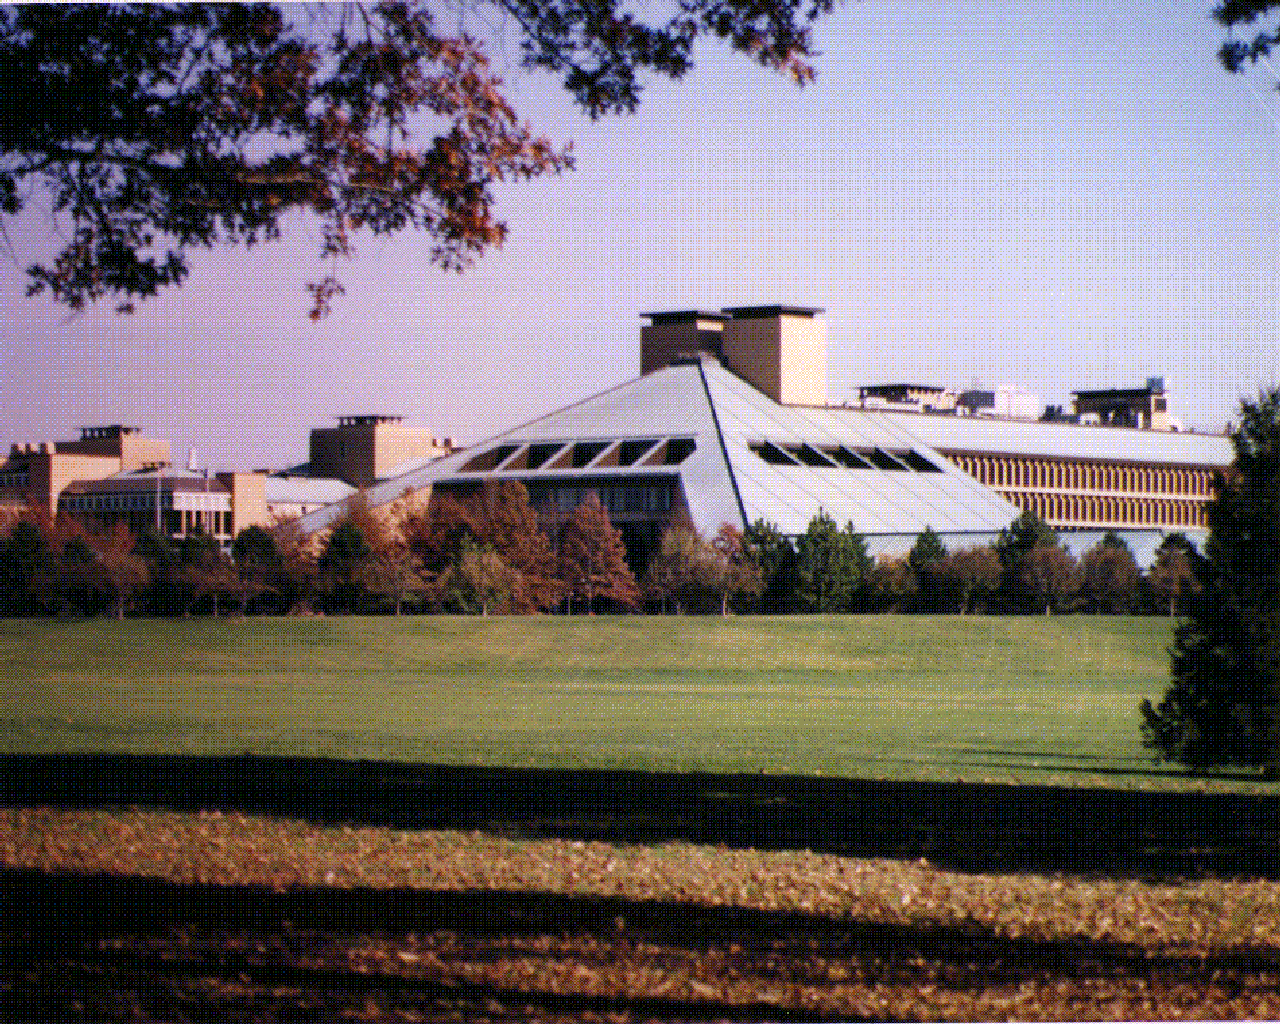
\includegraphics[width=0.6\textwidth]{assets/Lucent_HQ.png} 					\break
     		\break
     		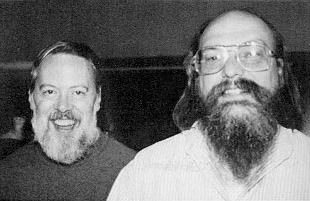
\includegraphics[width=0.6\textwidth]{assets/Ken_n_dennis.png}
     	\end{center}
		\end{column}
		
	\end{columns}
\end{frame}
%%---------------------------------------------------------------------

\subsection{Eksempler på brug af C}
\begin{frame}{Eksempler på brug af C}
	\begin{columns}
	
	\begin{column}{0.5\textwidth}
	\begin{itemize}
	\item{Kernen til dit Operativsystem er hovedsagligt skrevet i C}
	\item{C har inspireret mange sprog}
		\begin{itemize}
		\item{Swift}
		\item{Java}
		\item{PHP}
		\item{R}
		\end{itemize}
	\item{Compilers og interpreters er ofte skrevet i C!}
	\item{C bruges i indlejret elektronik i stor stil!}
	\end{itemize}
	\end{column}
	
	\begin{column}{0.5\textwidth}
	\begin{center}
		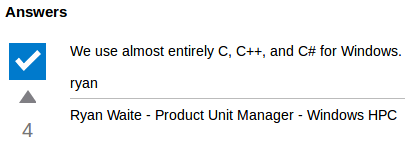
\includegraphics[width=0.7\textwidth]{assets/windows-kernel.png}
		\break
		
\includegraphics[width=0.7\textwidth]{assets/C-derivatives.png}
	\end{center}
	\end{column}
	
	\end{columns}
\end{frame}

\section{Et C-programs opbygning}
%%----------------------------------------------------------------------
\subsection{Et C-programs opbygning}
\begin{frame}[fragile]{Et C-programs opbygning}
	\begin{columns}
	
	\begin{column}{0.5\textwidth}
	
	\begin{itemize}
	\item{Linje 3:}
		\begin{itemize}
		\item{\bf{main()} er & hovedfunktionen}
		\end{itemize}
	\end{itemize}
	
	\begin{itemize}
	\item{Linje 6:}
		\begin{itemize}
		\item{Funktioner "returnerer" & ofte status til sidst}
		\end{itemize}
	\end{itemize}
	
	\begin{itemize}
	\item{Linje 1:}
		\begin{itemize}
		\item{Libraries med standardkomponenter}
		\end{itemize}
	\end{itemize}
	
	\begin{itemize}
	\item{Linje 5:}
		\begin{itemize}
		\item{printf() er en af dem. & Den skriver til konsollen}
		\end{itemize}
	\end{itemize}
	
	\end{column}
	
	\begin{column}{0.4\textwidth}
	\begin{lstlisting}
	#include <stdio.h>

	int main(void)
	{
		printf("Hello world\n");
		return 0;
	}
	\end{lstlisting}
	\end{column}
	
	\end{columns}
	
	\begin{center}
	Output:
	\lstset{language=bash, numbers=none}
	\begin{lstlisting}
	Hello world
	\end{lstlisting}
	\end{center}

\end{frame}
%%----------------------------------------------------------------------
\begin{frame}[fragile]{Et C-programs opbygning}
	\begin{columns}
	\begin{small}
	\begin{column}{0.5\textwidth}
	\begin{itemize}
	\item{Linje 3:}
		\begin{itemize}
		\item{Man kan deklarere variable}
		\end{itemize}
	\end{itemize}
	
	\begin{itemize}
	\item{Linje 10:}
		\begin{itemize}
		\item{Og lægge dem sammen}
		\end{itemize}
		\begin{itemize}
		\item{I en ny variabel}
		\end{itemize}
	\end{itemize}
	
	\begin{itemize}
	\item{Linje 11:}
		\begin{itemize}
		\item{Skrive dem ud, & formateret}
		\end{itemize}
	\end{itemize}
	\end{column}
	\end{small}
	
	\begin{column}{0.4\textwidth}
	\begin{lstlisting}
	#include <stdio.h>
	
	int a;
	int b;	
	
	int main(void)
	{
		a = 2;
		b = 3;
		int c = a + b;
		printf("%d + %d = %d\n", a, b, c);
		return 0;
	}
	\end{lstlisting}
	\end{column}
	
	\end{columns}
	\begin{center}
	Output:
	\lstset{language=bash, numbers=none}
	\begin{lstlisting}
	2 + 3 = 5 
	\end{lstlisting}
	\end{center}
\end{frame}

\section{Øvelseseksempler}
%%----------------------------------------------------------------------
\subsection{Opsætning af CodeLite}
\begin{frame}{Opsætning af CodeLite}
	\begin{itemize}
	\item{Nu skal vi have opsat CodeLite}
	\begin{itemize}
		\item{\url{https://downloads.codelite.org/}}
		\end{itemize}
	\item{Hvad man kalder et IDE}
		\begin{itemize}
		\item{Integrated Development Environment}
		\end{itemize}
	\item{Det gør vi live!}
	\end{itemize}
\end{frame}

%%----------------------------------------------------------------------
\subsection{Eksempel 1 - Hello World}
\begin{frame}{Eksempel 1 - Hello World}
	\begin{itemize}
	\item{Det første program hedder Hello World}
	\item{Det er en klassiker inden for programmering}
		\begin{itemize}
		\item{Første program man laver, så der er hul igennem}
		\end{itemize}
	\item{\color{link}\href{https://github.com/Iakop/C-Programmering-for-begyndere/tree/master/Del_1/Examples/1_Hello_World/main.c}{../Del\_1/Examples/1\_Hello\_World/main.c}}
	\item{Vi tager den i fællesskab!}
	\end{itemize}
\end{frame}

%%----------------------------------------------------------------------
\begin{frame}[fragile]{Eksempel 1 - Hello World}
	\begin{lstlisting}
	#include <stdio.h> 
	
	int main(int argc, char **argv)
	{
		printf("hello world\n");
		return 0;
	}
	\end{lstlisting}
	\begin{center}
	Output:
	\lstset{language=bash, numbers=none}
	\begin{lstlisting}
	hello world
	\end{lstlisting}
	\end{center}
\end{frame}

%%----------------------------------------------------------------------
\subsection{Eksempel 2 - Datatyper}
\begin{frame}{Eksempel 2 - Datatyper}
	\begin{itemize}
	\item{Vi skal lære forskellen på datatyper i C}
	\item{Der er en række forskellige:}
		\begin{itemize}
		\item{int - heltal/integer}
		\item{floating - floating point kommatal}
		\item{char - skrifttegn/character}
		\item{bool - sand/falsk (implementeret i stdbool.h)}
		\end{itemize}
	\item{\color{link}\href{https://github.com/Iakop/C-Programmering-for-begyndere/tree/master/Del_1/Examples/2_Datatypes/main.c}{../Del\_1/Examples/2\_Datatypes/main.c}}
	\item{Vi tager den i fællesskab!}
	\end{itemize}
\end{frame}

%%----------------------------------------------------------------------
\begin{frame}[fragile]{Eksempel 2 - Datatyper}
	\begin{lstlisting}
	#include <stdio.h>

	int main(int argc, char **argv)
	{
  		int a = 10; //integer
  		float b = 2.5; //float

		printf("an integer is a whole number. integer 'a' is: %d\n\n",a);
  		printf("floats can store decimals as well. float 'b' is : %f\n\n",b);
  		printf("we don't always want that many decimals though! you can adjust that like this %.2f\n\n",b);
  
  		char ch = 'A'; //char
  		printf("a character has several values, the character value is %c, and the integer value is %d\n\n",ch,ch);
		return 0;
	}
	\end{lstlisting}
\end{frame}

%%----------------------------------------------------------------------
\begin{frame}[fragile]{Eksempel 2 - Datatyper}
	\lstset{language=bash, numbers=none}
	\begin{center}
	Output:
	\lstset{language=bash, numbers=none}
	\begin{lstlisting}
	an integer is a whole number. integer 'a' is: 10

	floats can store decimals as well. float 'b' is : 2.500000

	we don't always want that many decimals though! you can adjust that like this 2.50

	a character has several values, the character value is A, and the integer value is 65

	\end{lstlisting}
	\end{center}
\end{frame}

%%----------------------------------------------------------------------
\subsection{Eksempel 3 - Matematik med Datatyper}
\begin{frame}{Eksempel 3 - Matematik med Datatyper}
	\begin{itemize}
	\item{Hvordan regnes med de forskellige datatyper?}
	\item{Vi ser lidt på basal aritmetik}
		\begin{itemize}
		\item{Multiplikation}
		\item{Division}
		\end{itemize}
	\item{Og hvordan variablene reagerer}
	\item{\color{link}\href{https://github.com/Iakop/C-Programmering-for-begyndere/tree/master/Del_1/Examples/3_Datatype_Math/main.c}{../Del\_1/Examples/3\_Datatype\_Math/main.c}}
	\item{Vi tager den i fællesskab!}
	\end{itemize}
\end{frame}

%%----------------------------------------------------------------------
\begin{frame}[fragile]{Eksempel 3 - Matematik med Datatyper}
	\lstset{basicstyle=\tiny}
	\begin{lstlisting}
	#include <stdio.h>

	int main(int argc, char **argv)
	{
  		int a = 10;
  		int b = 3;
  
  		printf("A quick way to do maths: %d * %d is %d\n\n", a,b,a*b);
  		
  		int c = a * b;

  		printf("displaying the math in varible c: %d * %d is %d\n\n",a,b,c);
  
  		c = a / b;
  
  		printf("wrong datatypes can cause some problems: %d / %d as en integer result: %d\n\n",a,b,c);
  
  		float d = 10;
  		float e = 3;
  		float f = d / e;
  
  		printf("Now with a float format specifier: %.1f / %.1f as a float result: %.2f\n\n",d,e,f);
  
		return 0;
	}
	\end{lstlisting}
\end{frame}

%%----------------------------------------------------------------------
\begin{frame}[fragile]{Eksempel 3 - Matematik med Datatyper}
	\lstset{language=bash, numbers=none, keywordstyle=\color{whiteee}}
	\begin{center}
	Output:
	\begin{lstlisting}
	A quick way to do maths: 10 * 3 is 30

	displaying the math in varible c: 10 * 3 is 30

	wrong datatypes can cause some problems: 10 / 3 as en integer result: 3

	Now with a float format specifier: 10.0 / 3.0 as a float result: 3.33

	\end{lstlisting}
	\end{center}
\end{frame}

%%----------------------------------------------------------------------
\subsection{Eksempel 4 - Input og Output}
\begin{frame}{Eksempel 4 - Input og Output}
	\begin{itemize}
	\item{Vores programmer har været meget ensidige}
		\begin{itemize}
		\item{Data har været "hardcoded"}
		\item{Vi har brug for input!}
		\end{itemize}
	\item{scanf() kan afhjælpe dette!}
		\begin{itemize}
		\item{Hører til i samme pakke som printf}
		\item{stdio.h}
		\end{itemize}
	\item{\color{link}\href{https://github.com/Iakop/C-Programmering-for-begyndere/tree/master/Del_1/Examples/4_Input_Output/main.c}{../Del\_1/Examples/4\_Input\_Output/main.c}}
	\item{Vi tager den i fællesskab!}
	\end{itemize}
\end{frame}

%%----------------------------------------------------------------------
\begin{frame}[fragile]{Eksempel 4 - Input og Output}
	\lstset{basicstyle=\tiny}
	\begin{lstlisting}
	#include <stdio.h>

	int main(int argc, char **argv)
	{
  		float input;

  		printf("Please input a number: "); //print input prompt
  		scanf("%f",&input); //take float value as input
  
  		printf("\nHere is your entered number: %.2f\n\n",input);
  
  		float input1;
  		float input2;
  		printf("enter two numbers to be multiplied, hit enter after each number:\n");
  		scanf("%f %f",&input1,&input2);

  		float result = input1 * input2;
  		printf("result: %.2f * %.2f = %.2f\n\n",input1,input2,result);
  
		return 0;
	}
	\end{lstlisting}
\end{frame}

%%----------------------------------------------------------------------
\begin{frame}[fragile]{Eksempel 4 - Input og Output}
	\lstset{language=bash, numbers=none, keywordstyle=\color{whiteee}}
	\begin{center}
	Output:
	\begin{lstlisting}
	Please input a number: 3

	Here is your entered number: 3.00

	enter two numbers to be multiplied, hit enter after each number:
	3
	3
	result: 3.00 * 3.00 = 9.00
	\end{lstlisting}
	\end{center}
\end{frame}

\section{Kreative Opgaver}
%%----------------------------------------------------------------------
\begin{frame}{Kreative Opgaver}
	\begin{itemize}
	\item{Der ligger kreative opgaver tilgængelige:}
		\begin{itemize}
		\item{\color{link}\href{https://github.com/Iakop/C-Programmering-for-begyndere/tree/master/Del_1/Exercises/C_exercises_1_dansk.pdf}{../Del\_1/Exercises/C\_exercises\_1\_dansk.pdf}}
		\end{itemize}
	\item{Der er hjælp at hente her på workshoppen}
	\item{God arbejdslyst! - Happy Hacking!}
	\end{itemize}
\end{frame}

\end{document}

%%\begin{frame}[fragile]
	%%\begin{lstlisting}
		%%#include <stdio.h>

		%%int main(void)
		%%{
		%%printf("Hello world\n");
		%%return 0;
		%%}
	%%\end{lstlisting}
%%\end{frame}